\chapter{Diseño}
\label{capdiseno}


\subsection{Diseño arquitectónico} \label{disenoarq}
Defina (si corresponde) los patrones de dise~no que usará. Incluya modelo de estructura
del sistema el cual debe reflejar el tipo de arquitectura especifica (cliente-servidor,
3 capas, SOA). Cada módulo debe estar trazado con respecto a los subsistemas identificados en el modelo de estructura.
De ser necesario incluya modelo de control.


\section{Diseño de interfaz} \label{disenoint}

Debido a que el siguiente sistema está destinado a una corporación especifica, nos resulta de vital importancia que la interfaz y la usabilidad de la herramienta sea agradable para los profesionales que trabajarán con ella.\\
Es por ello que el objetivo del diseño de la interfaz debe resultar en un sistema atractivo para los profesionales, y que la utilización del sistema no resulte difícil.\\
Además como el objetivo general de este Trabajo de Título es crear una herramienta que automatice, debemos tener un real cuidado con la interfaz, ya que podríamos tener el mejor código de programación y todos los requerimientos funcionales a la perfección, pero sin embargo si la interacción del usuario no es buena, el usuario preferirá realizar las apreciaciones como las realizaba previo a la creación de la herramienta.\\
A continuación se detalla el diseño de la interfaz con el qe el usuario se comunicará con la herramienta. 

\subsection{Estilos de interacción}

La interacción de los usuarios que utilizarán nuestra herramienta se produce mediante la manipulación directa de un navegador web. En donde los dos usuarios de nuestra herramienta que son, el administrador y usuario profesional poseerán diferentes sub-interfaces.


\subsection{Interfaz usuaria}

A continuación se presenta el diseño de la interfaz de usuario el cual se realizó con la herramienta Balsamiq Mckups 3. Cabe mencionar que se eligió realizar el diseño con esta herramienta debido a que sus representaciones entregan un balance entre la fidelidad y la velocidad del diseño. \\
Esta herramienta ofrece una representación sólida del diseño final donde se describen todos los componentes del sistema y se realiza de una manera rápida y sin tanto detalle. \\

La figura \ref{intinicio} muestra la interfaz inicial de nuestra herramienta la cual incluye una imagen representativa del PPF Aitué, el login de usuario (Profesional o Administrador).\\

\begin{figure}[h]
	\label{intinicio}
	\begin{center}
		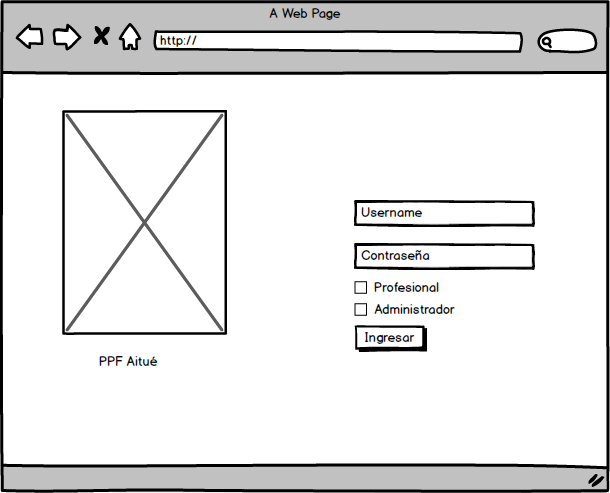
\includegraphics[scale=0.5]{imagenes/login.png}
	\end{center}
	\caption{Interfaz de inicio de la herramienta.}
\end{figure}

\clearpage
\newpage

La figura \ref{intadm} muestra la interfaz inicial luego de ingresar con la cuenta de administrador de nuestra herramienta la cual incluye una imagen representativa del PPF Aitué, el ícono con la opción de crear un nuevo usuario, modificar un nuevo usuario, ingresar al sistema y finalmente la opción de eliminar un usuario del sistema.\\


\begin{figure}[h]
	\label{intadm}
	\begin{center}
		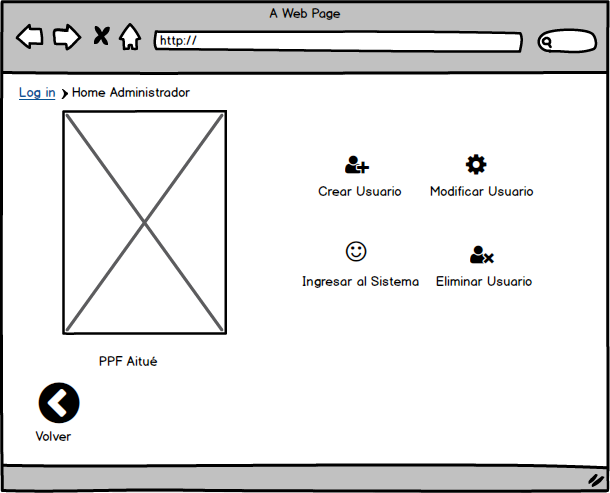
\includegraphics[scale=0.5]{imagenes/intadm.png}
	\end{center}
	\caption{Interfaz que muestra el inicio luego de ingresar como administrador.}
\end{figure}

\clearpage
\newpage

La figura \ref{newuser} muestra la interfaz luego que el administrador seleccione la opción crear usuario. Esta interfaz cuenta con un formulario que se compone de:
\begin{itemize}
	\item Nombre de usuario
	\item Contraseña
	\item Repetir contraseña
	\item Rut
	\item Mail
	\item Tipo de usuario (Psicologo o Asistente Social)
\end{itemize}

Además de una imagen representativa y en la parte inferior  los botones "Crear Usuario" y "Volver"\\

\begin{figure}[htb]
	\label{newuser}
	\begin{center}
		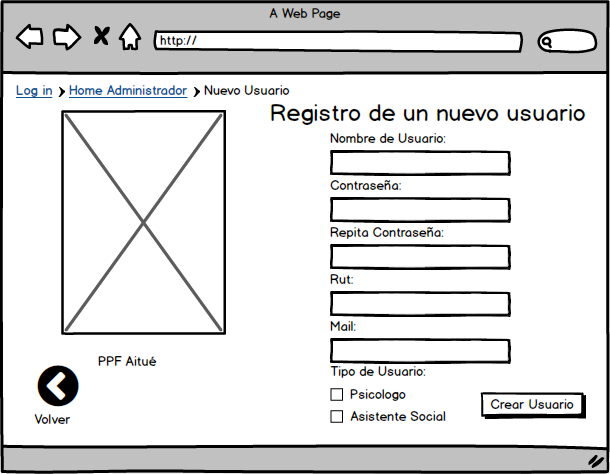
\includegraphics[scale=0.5]{imagenes/newuser.png}
	\end{center}
	\caption{Interfaz que muestra el formulario de ingreso de un nuevo usuario al sistema.}
\end{figure}

\clearpage
\newpage

La figura \ref{moduser1} muestra la interfaz luego que el administrador selecciona la opción modificar usuario, en esta interfaz se despliegan todos los usuarios almacenados en el sistema y en la parte inferior de esta lista, se muestra el botón "Modifiar usuario". \\


\begin{figure}[htb]
	\label{moduser1}
	\begin{center}
		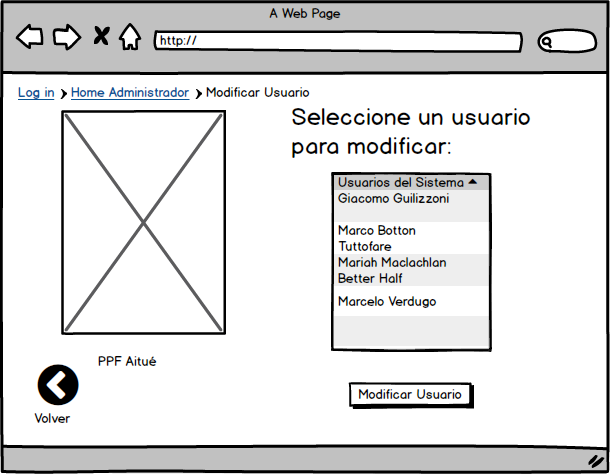
\includegraphics[scale=0.5]{imagenes/moduser1.png}
	\end{center}
	\caption{Interfaz que muestra el inicio luego de ingresar como administrador.}
\end{figure}

\clearpage
\newpage

La figura \ref{moduser} muestra la interfaz luego que el administrador seleccione la opción modificar usuario y selecciona un usuario a modificar. Esta interfaz cuenta los campos editables de:
\begin{itemize}
	\item Nombre de usuario
	\item Contraseña
	\item Mail
	\item Rut
	\item Mail
	\item Tipo de usuario (Psicologo o Asistente Social)
\end{itemize}

Además de una imagen representativa y en la parte inferior  los botones "Crear Usuario" y "Volver".\\

\begin{figure}[htb]
	\label{moduser}
	\begin{center}
		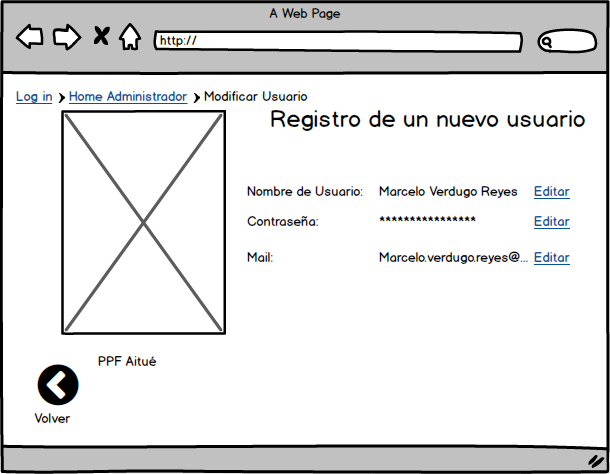
\includegraphics[scale=0.5]{imagenes/moduser.png}
	\end{center}
	\caption{Interfaz que muestra los campos editables luego de seleccionar un usuario a modificar.}
\end{figure}

\clearpage
\newpage

La figura \ref{bienvenido} muestra la interfaz luego que el administrador selecciona "Ingresar al sistema" o bien posteriormente que el profesional realiza su login.\\
En esta interfaz se muestran dos íconos representativos de la herramientas NCFAS y de la herramienta CAT-A, donde CAT-A es la herramienta del Trabajo de Título a realizar de Jean Pierre Peña. \\
Además una imagen representativa y en la parte inferior el botón "Volver".\\

\begin{figure}[htb]
	\label{bienvenido}
	\begin{center}
		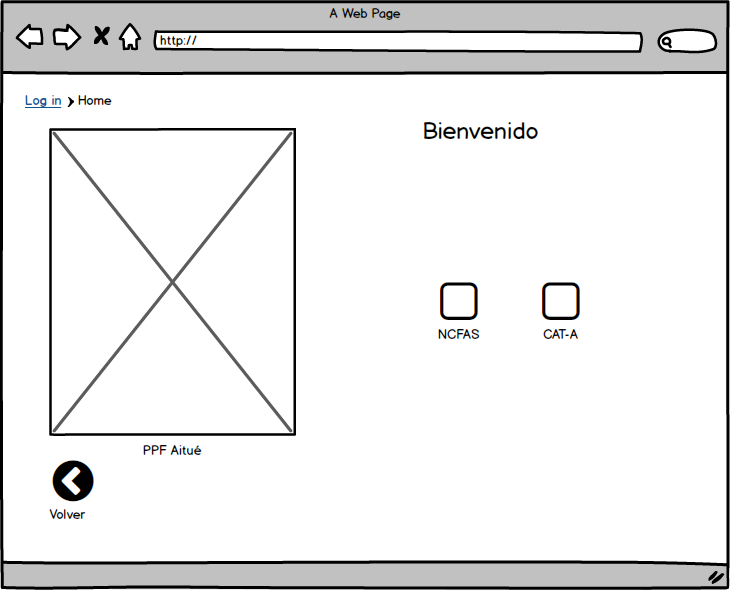
\includegraphics[scale=0.5]{imagenes/bienvenido.png}
	\end{center}
	\caption{Interfaz que muestra el inicio del sistema.}
\end{figure}

\clearpage
\newpage

La figura \ref{inicioncfas} muestra la interfaz luego que el administrador o el profesional ingresan a la herramienta NCFAS. Esta interfaz de bienvenida a la herramienta NCFAS, muetra en el costado izquierdo las posibles tareas que pueden ser realizadas por el administrador y por el profesional dentro de la herramienta NCFAS.\\

Además de una imagen representativa y de los botones "Crear Usuario" y "Volver".\\

\begin{figure}[htb]
	\label{inicioncfas}
	\begin{center}
		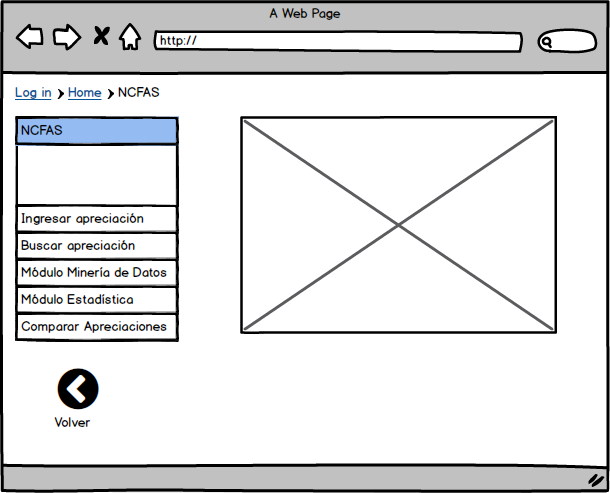
\includegraphics[scale=0.5]{imagenes/inicioncfas.png}
	\end{center}
	\caption{Interfaz que muestra el inicio luego de ingresar a la herramienta NCFAS.}
\end{figure}

\clearpage
\newpage

La figura \ref{ncfasguardados} muestra las apreciaciones guardadas en el sistema las cuales al ser seleccionadas por el administrador o por el profesional, estas pueden ser modificadas, comparadas, o bien encontrar información útil utilizando en ellas, técnicas de minería de datos o de estadística descriptiva.\\

\begin{figure}[htb]
	\label{ncfasguardados}
	\begin{center}
		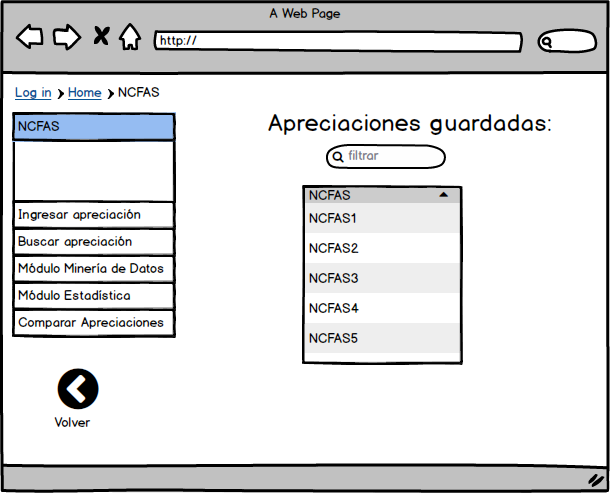
\includegraphics[scale=0.5]{imagenes/ncfasguardados.png}
	\end{center}
	\caption{Interfaz que muestra el inicio luego de ingresar a la herramienta NCFAS.}
\end{figure}

\clearpage
\newpage

La figura \ref{dimncfas} muestra las distintas dimensiones que componen la herramienta NCFAS. 
Además de las diferentes opciones que puede realizar el profesional o el administrador en el costado izquierdo, junto con el botón volver en la parte inferior izquierda.\\

\begin{figure}[htb]
	\label{dimncfas}
	\begin{center}
		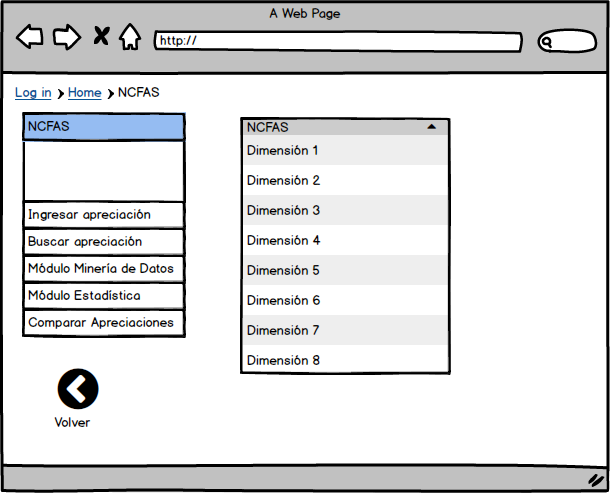
\includegraphics[scale=0.5]{imagenes/dimncfas.png}
	\end{center}
	\caption{Interfaz que muestra el inicio luego de ingresar a la herramienta NCFAS.}
\end{figure}

\clearpage
\newpage

La figura \ref{itmncfas2} muestra los distintos ítems que componen dimensiones de la herramienta NCFAS. 
Además de las diferentes opciones que puede realizar el profesional o el administrador en el costado izquierdo, junto con el botón volver en la parte inferior izquierda.\\

\begin{figure}[htb]
	\label{itmncfas2}
	\begin{center}
		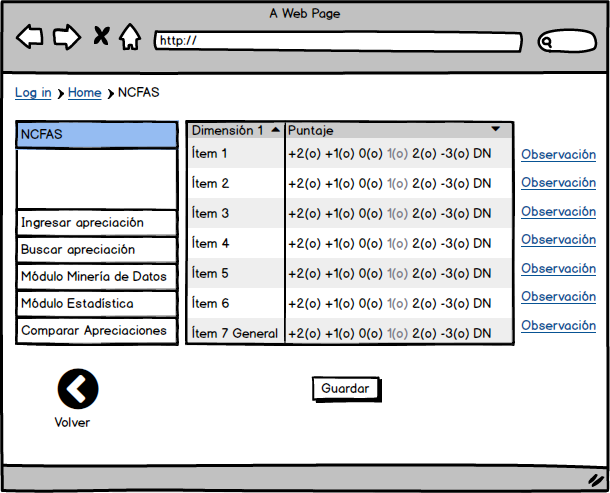
\includegraphics[scale=0.5]{imagenes/itmncfas.png}
	\end{center}
	\caption{Interfaz que muestra el inicio luego de ingresar a la herramienta NCFAS.}
\end{figure}

\clearpage
\newpage

\section{Diseño lógico} \label{disenolog}



\subsubsection{Esquemas de navegación}

\clearpage
\newpage

\subsection{Diagrama de clases}

\clearpage
\newpage

\subsection{Caso de uso reales}

En la siguiente sección se detallara la experiencia que tendrá el usuario con el sistema, mostrando cada funcionalidad. En donde los números indica donde el usuario puede interactuar con el sistema y la letra indica la interfaz a la cual se hace referencia.\\

\begin{figure}[htb]
	\label{inicioadm2}
	\begin{center}
		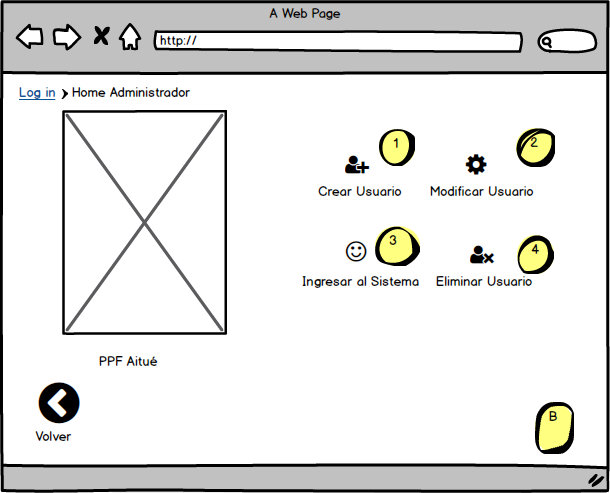
\includegraphics[scale=0.3]{imagenes/inicioadm2.png}
	\end{center}
	\caption{Interfaz que muestra el inicio luego de ingresar a la herramienta NCFAS.}
\end{figure}

\begin{figure}[htb]
	\label{formuser}
	\begin{center}
		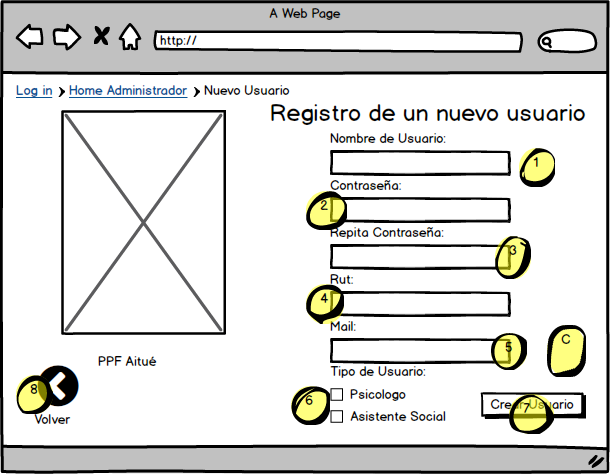
\includegraphics[scale=0.3]{imagenes/formuser.png}
	\end{center}
	\caption{Interfaz que muestra el formulario para crear un usuario.}
\end{figure}

\begin{figure}[htb]
	\label{newuseralt}
	\begin{center}
		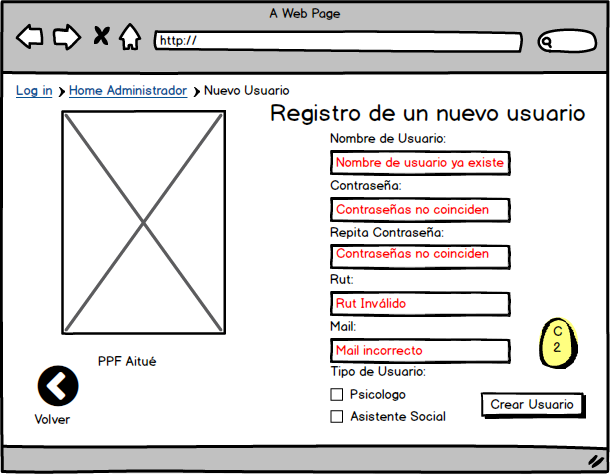
\includegraphics[scale=0.3]{imagenes/newuseralt.png}
	\end{center}
	\caption{Interfaz que muestra el formulario para crear un usuario.}
\end{figure}

\begin{table}
	\centering
	\begin{tabular}{|p{3cm}|p{3cm}|p{2.3cm} |p{5cm}|}
		\hline \textbf{Caso de Uso} & Crear Usuario & \textbf{ID} & CDU1 \\ 
		\hline \textbf{Actores} & Administrador & \textbf{Tipo} & Primario \\ 
		\hline \textbf{Pre-condición} & - & \textbf{Descripción} & Permite crear un usuario\\
		\hline \textbf{Ref. Cruzadas} & RF1 & \textbf{Resumen} & El administrador crea los usuarios asignando un respectivo nombre, e-mail, contraseña y perfil.\\ 
		\hline
	\end{tabular}  
	
	\begin{tabular}{|p{8cm}|p{6cm}|}
		
		\multicolumn{2}{|c|}{\textbf{Curso normal de eventos}} \\
		\hline \textbf{Actor} & \textbf{Sistema} \\ 
		\hline 1. Este caso de uso comienza cuando el administrador debe crear un usuario para el sistema y presiona (1B). & 2.El sistema solicita al administrador el nombre de usuario (1C), e-mail (2C), contraseña(3C) que se confirme la contraseña (4C)y que seleccione el nuevo usuario (Psicólogo o Asistente social)(5C)  \\ 
		3. El administrador ingresa lo solicitado y presiona el botón "Crear Usuario" (7C) & 4. El sistema valida lo ingresado por el administrador y crea el nuevo usuario. \\
		& 5. El sistema guarda el nuevo usuario y permite al administrador crear un nuevo usuario o bien ingresar al sistema. \\
		\hline
		\multicolumn{2}{|c|}{\textbf{Curso alternativo de eventos}} \\
		\hline
		\multicolumn{2}{|p{12cm}|}{4. El sistema valida los datos ingresados por el administrador pero estos no son válidos y vuelve al paso 3 y muestra los errores (C2).} \\
		\hline
	\end{tabular}
	\caption{Tabla del caso de uso expandido de Crear Usuario}
	\label{tabcdu1.1}
\end{table}
\clearpage
\begin{figure}[h!]
	\label{moduser2}
	\begin{center}
		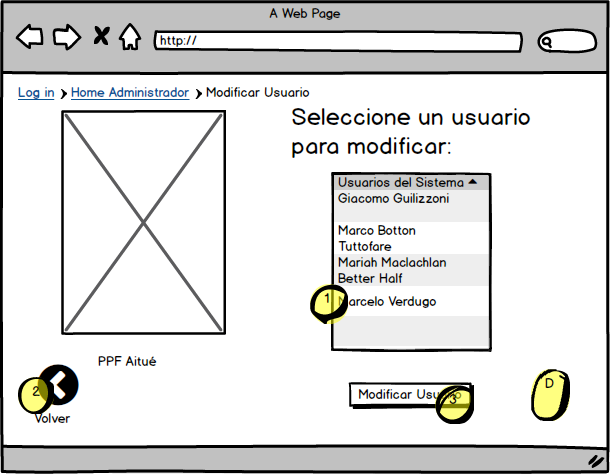
\includegraphics[scale=0.3]{imagenes/moduser2.png}
	\end{center}
	\caption{Interfaz que muestra los usuarios del sistema que se pueden modificar.}
\end{figure}
\begin{figure}[h!]
	\label{moduser3}
	\begin{center}
		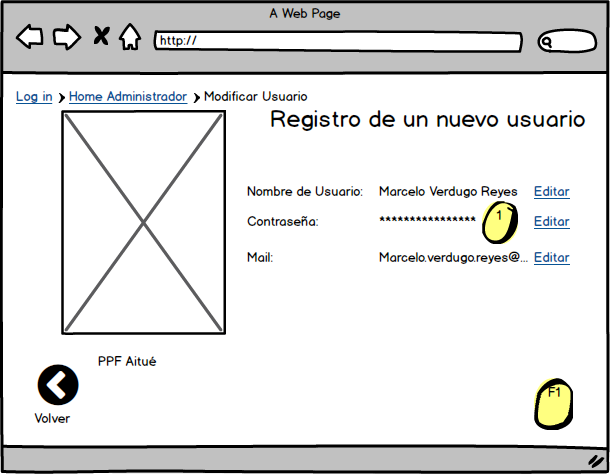
\includegraphics[scale=0.3]{imagenes/moduser3.png}
	\end{center}
	\caption{Interfaz que muestra los campos modificables del usuario.}
\end{figure}
\begin{figure}[h!]
	\label{moduser4}
	\begin{center}
		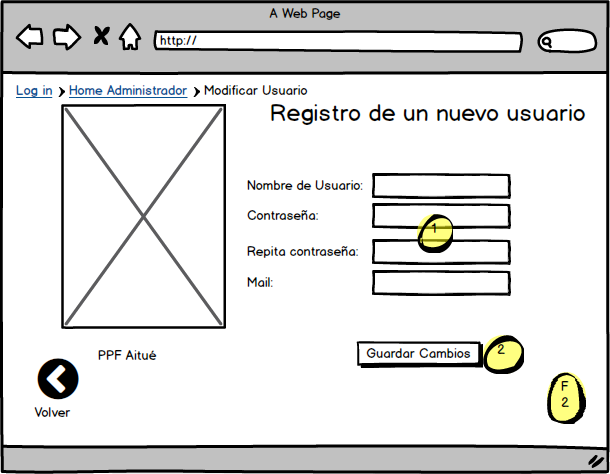
\includegraphics[scale=0.3]{imagenes/moduser4.png}
	\end{center}
	\caption{Interfaz que muestra los campos modificables del usuario.}
\end{figure}

\begin{figure}[h!]
	\label{moduser5}
	\begin{center}
		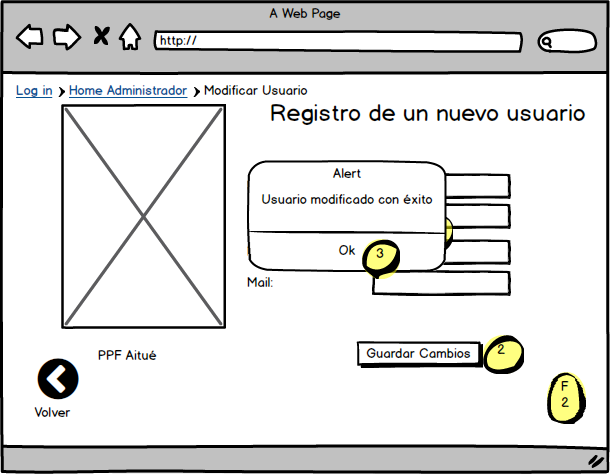
\includegraphics[scale=0.3]{imagenes/moduser5.png}
	\end{center}
	\caption{Interfaz que muestra los campos modificables del usuario.}
\end{figure}

\begin{figure}[h!]
	\label{moduser6}
	\begin{center}
		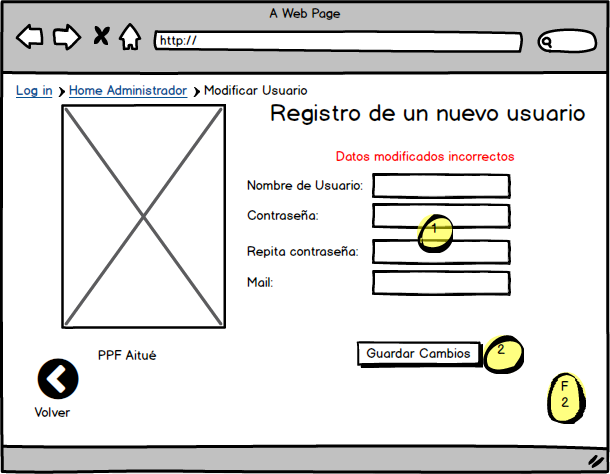
\includegraphics[scale=0.3]{imagenes/moduser6.png}
	\end{center}
	\caption{Interfaz que muestra los campos modificables del usuario.}
\end{figure}

\begin{table}
	\centering
	\begin{tabular}{|p{3cm}|p{3cm}|p{2cm} |p{3cm}|}
		\hline \textbf{Caso de Uso} & Modificar Usuario & \textbf{ID} & CDU2 \\ 
		\hline \textbf{Actores} & Administrador & \textbf{Tipo} & Opcional \\ 
		\hline \textbf{Pre-condición} & Crear un usuario & \textbf{Descripción} & Permite modificar un usuario creado anteriormente \\
		\hline \textbf{Ref. Cruzadas} & RF1 & \textbf{Resumen} & El administrador modifica un usuario creado anteriormente.\\ 
		\hline
	\end{tabular}  
	
	\begin{tabular}{|p{6cm}|p{6cm}|}
		
		\multicolumn{2}{|c|}{\textbf{Curso normal de eventos}} \\
		\hline \textbf{Actor} & \textbf{Sistema} \\ 
		\hline 1. Este caso de uso comienza cuando el administrador desea modificar un usuario creado anteriormente, seleccionando la opción modificar usuario (2B) \ref{inicioadm2}. & 2. El sistema muestra los usuarios guardados (D) \ref{moduser2}. \\ 
		3. El administrador selecciona al usuario que desea modificar(1D) \ref{moduser2} . & 4. El sistema muestra las opciones a modificar del usuario (F1) \ref{moduser3}.\\
		5. El administrador selecciona los campos a modificar (1F1) \ref{moduser2}. & 6. El sistema cambia y se adapta para recibir text imput (F2) \ref{moduser4} \\
		7. El administrador guarda las modificaciones (2F2) \ref{moduser4}. & 8. El sistema valida las modificaciones y guarda nuevamente el usuario modificado y muestra el alert (F2) \ref{moduser5} \\
		\hline
		\multicolumn{2}{|c|}{\textbf{Curso alternativo de eventos}} \\
		\hline
		\multicolumn{2}{|p{12cm}|}{7. El sistema valida los datos ingresados por el administrador pero estos no son válidos y vuelve al paso 5 \ref{moduser6}. } \\
		\hline
	\end{tabular}
	\caption{Tabla del caso de uso expandido de Modificar Usuario}
	\label{tabcdu22}
\end{table}

\clearpage

\begin{figure}[h!]
	\label{elimuser2}
	\begin{center}
		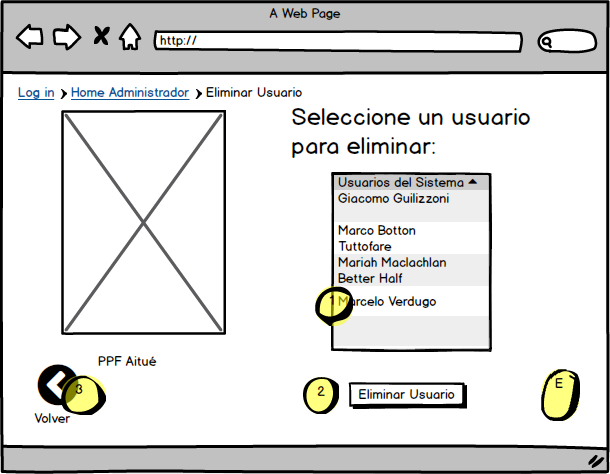
\includegraphics[scale=0.3]{imagenes/elimuser2.png}
	\end{center}
	\caption{Interfaz que muestra los campos modificables del usuario.}
\end{figure}

\begin{figure}[h!]
	\label{elimuser4}
	\begin{center}
		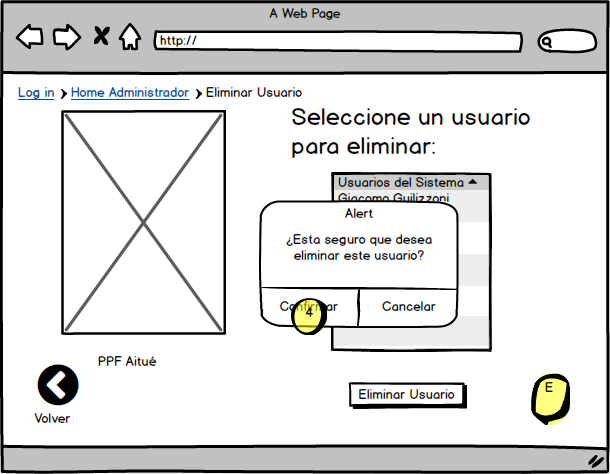
\includegraphics[scale=0.3]{imagenes/elimuser4.png}
	\end{center}
	\caption{Interfaz que muestra los campos modificables del usuario.}
\end{figure}

\clearpage

\begin{figure}[h!]
	\label{elimuser5}
	\begin{center}
		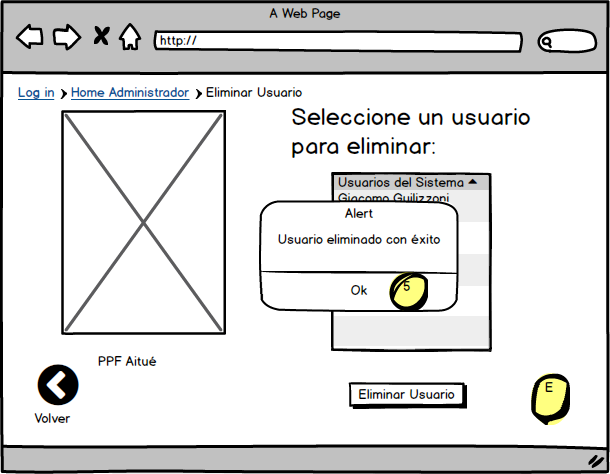
\includegraphics[scale=0.3]{imagenes/elimuser5.png}
	\end{center}
	\caption{Interfaz que muestra los campos modificables del usuario.}
\end{figure}

\begin{table}
	\centering
	\begin{tabular}{|p{3cm}|p{3cm}|p{2cm} |p{3cm}|}
		\hline \textbf{Caso de Uso} & Eliminar Usuario & \textbf{ID} & CDU3 \\ 
		\hline \textbf{Actores} & Administrador & \textbf{Tipo} & Opcional \\ 
		\hline \textbf{Pre-condición} & Crear un usuario & \textbf{Descripción} & Permite eliminar un usuario creado anteriormente \\
		\hline \textbf{Ref. Cruzadas} & RF1 & \textbf{Resumen} & El administrador elimina un usuario creado anteriormente.\\ 
		\hline
	\end{tabular}  
	\begin{tabular}{|p{6cm}|p{6cm}|}
		\multicolumn{2}{|c|}{\textbf{Curso normal de eventos}} \\
		\hline \textbf{Actor} & \textbf{Sistema} \\ 
		\hline 1. Este caso de uso comienza cuando el administrador desea eliminar un usuario creado anteriormente, seleccionando la opción eliminar usuario.(4B) \ref{inicioadm2} & 2. El sistema muestra los usuarios guardados (E) \ref{elimuser2} \\ 
		3. El administrador selecciona al usuario que desea eliminar.(1E) \ref{elimuser2} & \\
		4. El usuario presiona el botón "Eliminar Usuario" (2E) \ref{elimuser2} & 5. El sistema envía una alerta para que el administrador confirme que realmente desea eliminar el usuario seleccionado. \ref{elimuser4} \\
		6. El administrador confirma la eliminación.(4E) \ref{elimuser4} & 7. El sistema elimina al usuario y muestra una alerta (5E) \ref{elimuser5}. \\
		\hline
		\multicolumn{2}{|c|}{\textbf{Curso alternativo de eventos}} \\
		\hline
		\multicolumn{2}{|p{12cm}|}{5. El administrador cancela la eliminación del usuario y vuelve al paso 3. } \\
		\hline
	\end{tabular}
	\caption{Tabla del caso de uso expandido de Eliminar Usuario}
	\label{tabcdu33}
\end{table}

\clearpage

\begin{figure}[h!]
	\label{ncfas3}
	\begin{center}
		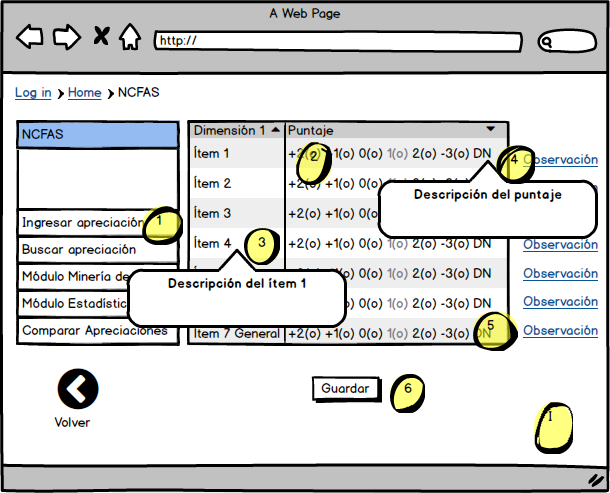
\includegraphics[scale=0.3]{imagenes/ncfas3.png}
	\end{center}
	\caption{Interfaz que muestra los campos modificables del usuario.}
\end{figure}

\begin{figure}[h!]
	\label{ncfas4}
	\begin{center}
		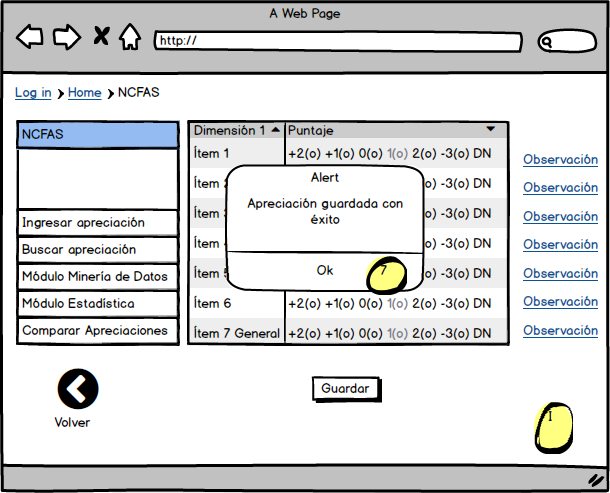
\includegraphics[scale=0.3]{imagenes/ncfas4.png}
	\end{center}
	\caption{Interfaz que muestra los campos modificables del usuario.}
\end{figure}


\begin{table}[h!]
	\centering
	\begin{tabular}{|p{2cm}|p{3cm}|p{2cm}|p{4cm}|}
		\hline \textbf{Caso de Uso} & Ingresar NCFAS & \textbf{ID} & CDU4 \\ 
		\hline \textbf{Actores} & Profesional a cargo- Administrador & \textbf{Tipo} & Primario \\ 
		\hline \textbf{Pre-condición} & - & \textbf{Descripción} & Permite ingresar una apreciación familiar mediante la herramienta NCFAS Digital \\
		\hline \textbf{Ref. Cruzadas} & RF2-RF3-RNF11 & \textbf{Resumen} & EL profesional a cargo o el administrador, luego de recopilar información necesaria de la familia, ordena y califica la información por medio de la herramienta NCFAS.\\ 
		\hline
	\end{tabular}  
	\begin{tabular}{|p{6cm}|p{6cm}|}
		
		\multicolumn{2}{|c|}{\textbf{Curso normal de eventos}} \\
		\hline \textbf{Actor} & \textbf{Sistema} \\ 
		\hline 1. Este caso de uso comienza cuando el profesional a cargo desea ingresa una nueva apreciación familiar presionando "Ingresar apreciación" (1I) \ref{ncfas3}. & 2. El sistema despliega la herramienta NCFAS Digital que se observa en (I) \ref{ncfas3}.  \\ 
		3. El profesional a cargo califica cada ítem, donde además puede ver los descriptores asociados a cada ítem (3I) y a cada puntaje asociado (4I) \ref{ncfas3}.&  \\
		4. El profesional guarda todo su progreso (6I) \ref{ncfas3}. & 5. El sistema guarda y almacena la apreciación completa y envía un alert al usuario informando que se guardó con éxito. (7C) \ref{ncfas4} \\
		\hline
		\multicolumn{2}{|c|}{\textbf{Curso alternativo de eventos}} \\
		\hline
		\multicolumn{2}{|p{12cm}|}{-} \\
		\hline
	\end{tabular}
	\caption{Tabla del caso de uso expandido de NCFAS Digital}
	\label{tabcdu44}
\end{table}

\clearpage

\begin{figure}[h!]
	\label{generainfo}
	\begin{center}
		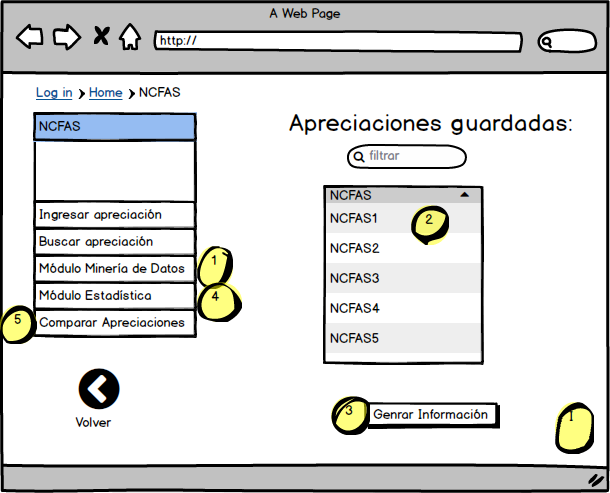
\includegraphics[scale=0.3]{imagenes/generainfo.png}
	\end{center}
	\caption{Interfaz para generar información útil a partir de las NCFAS.}
\end{figure}

\begin{figure}[h!]
	\label{estadistic}
	\begin{center}
		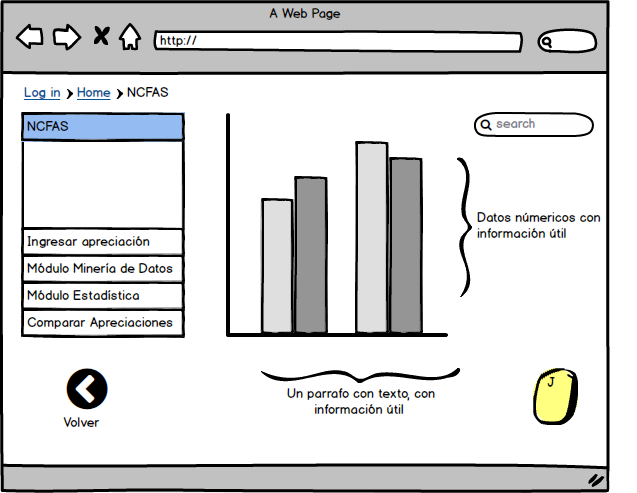
\includegraphics[scale=0.3]{imagenes/estadistic.png}
	\end{center}
	\caption{Interfaz que muestra la información utilizando técnicas de estadística descriptiva.}
\end{figure}

\begin{table}
	\centering
	\begin{tabular}{|p{6cm} |p{6cm}|}
		\hline \textbf{Caso de Uso} & Visualizar Información Estadística Descriptiva \\ 
		\hline \textbf{ID} & CDU6 \\ 
		\hline \textbf{Actores} & Profesional a cargo \\ 
		\hline \textbf{Tipo} & Opcional \\ 
		\hline \textbf{Pre-condición} & Existan apreciaciones guardadas \\ 
		\hline \textbf{Descripción} & Permite que el profesional a cargo visualice información con técnicas de Estadística Descriptiva \\
		\hline \textbf{Ref. Cruzadas} & RF4 - RF6 \\ 
		\hline
		\multicolumn{2}{|c|}{\textbf{Resumen}} \\
		\hline
		\multicolumn{2}{|p{12cm}|}{El profesional a cargo podrá visualizar la información , mediante técnicas de estadística descriptiva.} \\
		\hline 
	\end{tabular}  
	\begin{tabular}{|p{6cm}|p{6cm}|}
		\multicolumn{2}{|c|}{\textbf{Curso normal de eventos}} \\
		\hline \textbf{Actor} & \textbf{Sistema} \\ 
		\hline 1. Este caso de uso comienza cuando el profesional a cargo desea visualizar información mediante el módulo de estadística descriptiva presionando (1I) \ref{generainfo}. & 2.El sistema despliega las NCFAS guardadas para que el profesional seleccione una para generar la información.  \\ 
		3. El profesional a cargo selecciona una NCFAS (2I) \ref{generainfo}. & 4.El sistema despliega la información.(J) \ref{estadistic}  \\ 
		\hline
		\multicolumn{2}{|c|}{\textbf{Curso alternativo de eventos}} \\
		\hline
		\multicolumn{2}{|p{12cm}|}{ - } \\
		\hline
	\end{tabular}
	\caption{Tabla del caso de uso expandido de Visualizar Información Módulo Estadística Descriptiva}
	\label{tabcdu66}

\end{table}
\clearpage


\begin{figure}[h!]
	\label{min}
	\begin{center}
		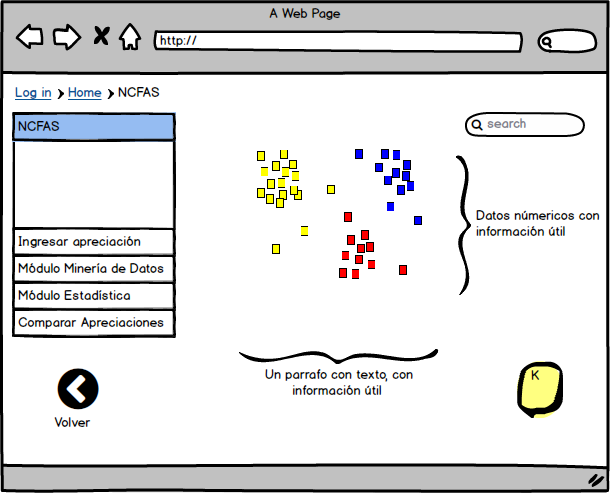
\includegraphics[scale=0.4]{imagenes/min.png}
	\end{center}
	\caption{Interfaz que muestra la información.}
\end{figure}

\begin{table}
	\centering
	\begin{tabular}{|p{6cm} |p{6cm}|}
		\hline \textbf{Caso de Uso} & Visualizar Información \\ 
		\hline \textbf{ID} & CDU7 \\ 
		\hline \textbf{Actores} & Profesional a cargo \\ 
		\hline \textbf{Tipo} & Opcional \\ 
		\hline \textbf{Pre-condición} & - \\ 
		\hline \textbf{Descripción} & Permite que el profesional a cargo visualice información con técnicas de Minería de Datos \\
		\hline \textbf{Ref. Cruzadas} & RF4 - RF6 \\ 
		\hline
		\multicolumn{2}{|c|}{\textbf{Resumen}} \\
		\hline
		\multicolumn{2}{|p{12cm}|}{El profesional a cargo podrá visualizar información mediante técnicas de minería de datos.} \\
		\hline 
	\end{tabular}  
	\begin{tabular}{|p{6cm}|p{6cm}|}
		\multicolumn{2}{|c|}{\textbf{Curso normal de eventos}} \\
		\hline \textbf{Actor} & \textbf{Sistema} \\ 
		\hline 1. Este caso de uso comienza cuando el profesional a cargo desea visualizar información mediante el módulo de minería de datos, presionando (4I) \ref{generainfo}. & 2.El sistema despliega las NCFAS guardadas para que el profesional seleccione una para generar la información.  \\ 
	El profesional a cargo selecciona una NCFAS (2I) \ref{generainfo}. & 4.El sistema despliega la información.(J) \ref{min}. \\
		\hline
		\multicolumn{2}{|c|}{\textbf{Curso alternativo de eventos}} \\
		\hline
		\multicolumn{2}{|p{12cm}|}{ - } \\
		\hline
	\end{tabular}
	\caption{Tabla del caso de uso expandido de Visualizar Información Módulo Minería de Datos}
	\label{tabcdu77}
\end{table}
\clearpage


\begin{figure}[h!]
	\label{compara}
	\begin{center}
		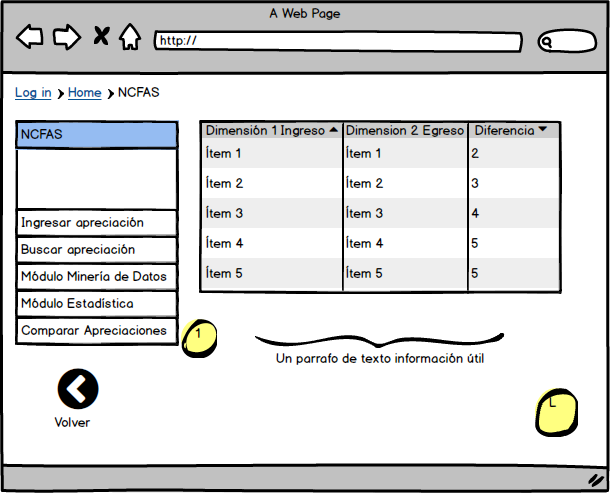
\includegraphics[scale=0.3]{imagenes/compara.png}
	\end{center}
	\caption{Interfaz que muestra la NCFAS de ingreso comparada con la NCFAS de egreso.}
\end{figure}

\begin{table}
	\centering
	\begin{tabular}{|p{6cm} |p{6cm}|}
		\hline \textbf{Caso de Uso} & Comparar NCFAS Digitales \\ 
		\hline \textbf{ID} & CDU9 \\ 
		\hline \textbf{Actores} & Profesional a cargo \\ 
		\hline \textbf{Tipo} & Opcional \\ 
		\hline \textbf{Pre-condición} & EL sistema debe tener NCFAS Digitales almacenados \\ 
		\hline \textbf{Descripción} & Permite comparar dos NCFAS(Ingreso v/s egreso) \\
		\hline \textbf{Ref. Cruzadas} & RF5 \\ 
		\hline
		\multicolumn{2}{|c|}{\textbf{Resumen}} \\
		\hline
		\multicolumn{2}{|p{12cm}|}{El profesional a cargo podrá comparar NCFAS Digitales dentro del sistema.} \\
		
	\end{tabular}  
	\begin{tabular}{|p{6cm}|p{6cm}|}
		\multicolumn{2}{|c|}{\textbf{Curso normal de eventos}} \\
		\hline \textbf{Actor} & \textbf{Sistema} \\ 
		\hline 1. Este caso de uso comienza cuando el profesional a cargo desea comparar apreciaciones familiares, presionando (5I) \ref{generainfo} & 2.El sistema despliega las NCFAS que puede seleccionar para comparar (Las que tengan una apreciación de ingreso y egreso).  \\ 
		3. El profesional a cargo selecciona las NCFAS que desea comparar, presionando (2I) \ref{generainfo}.& 4. El sistema despliega información acerca de los ítems que más variaron entre el NCFAS de ingreso v/s el NCFAS de egreso.(L) \ref{compara} \\
		\hline
		\multicolumn{2}{|c|}{\textbf{Curso alternativo de eventos}} \\
		\hline
		\multicolumn{2}{|p{12cm}|}{ - } \\
		\hline
	\end{tabular}
	\caption{Tabla del caso de uso expandido de Comparar NCFAS Digitales}
	\label{tabcdu99}
\end{table}

\clearpage

\section{Diseño de datos}  \label{disenodat}

En esta sección se detalla la creación de los archivos necesarios para poder almacenar los datos de las apreciaciones familiares y, posteriormente llevar a cabo las técnicas de minería de datos y estadística descriptiva. 

\subsection{Archivo ARFF}

En la herramienta NCFAS existen 8 dimensiones en dónde cada una de estas se compone de diferentes ítems, a su vez, cada ítem puede ser calificado con distintos valores, los que son:

\begin{itemize}
	\item NA (No aplica): Cuando no es necesario evaluar este ítem
	\item +2: El cual indica, una Clara Fortaleza 
	\item +1: El cual indica, una leve Fortaleza
	\item 0: El cual indica, una Linea de Base Adecuado
	\item -1: El cual indica, una Problema Leve
	\item -2: El cual indica, una clara Problema Moderado
	\item -3: El cual indica, una clara Problema Serio
	\item DN (Desconocido): Cuando se desconoce que valor otorgar a este ítem
\end{itemize}

Un ejemplo de una dimensión con sus respectivos ítem es la Figura \ref{escalaejem}.\\

\begin{figure}[h!]
	\label{escalaejem}
	\begin{center}
		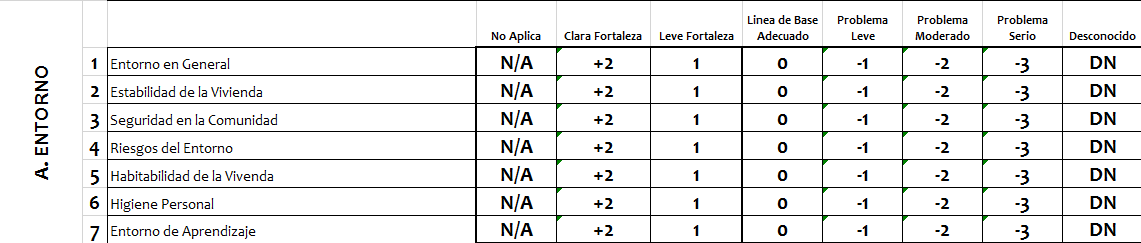
\includegraphics[scale=0.4]{imagenes/escalaejem.png}
	\end{center}
	\caption{Ejemplo de la dimensión "ENTORNO" con sus respectivos ítems.}
\end{figure}

\subsubsection{Representación ARFF}

La forma en la que será representado lo que se muestra en la Figura \ref{escalaejem} se realizará con un archivo ARFF, este archivo que sus siglas en inglés significan (Attribute-Relation File Format), es un archivo de texto ASCII que describe una lista de instancias que comparten un conjunto de atributos.\\

Un archivo ARFF se compone de dos secciones. La primera sección que es la cabecera de la información y la segunda que son los datos. La cabecera contiene los nombres de las relaciones, una lista de atributos y sus tipos. Este archivo se almacenará en una carpeta con el nombre de la familia a evaluar, seguido por un identificador. Dentro de esta carpeta encontraremos 9 tipos de archivos ARFF. \\

El cual cada uno de estos representará la información obtenida de cada dimensión y el noveno archivo ARFF contendrá la calificación total de cada dimensión evaluada.\\
Los datos que contendrá nuestro archivo ARFF serán los siguientes:

\begin{figure}[htb]
	\label{cabecera}
	\begin{center}
		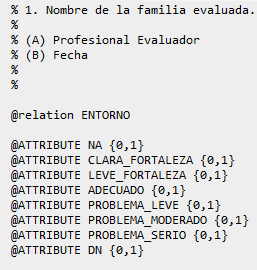
\includegraphics[scale=0.7]{imagenes/cabecera.png}
		\caption{Ejemplifica la forma en que los datos serán representados en nuestro sistema.}
	\end{center}
\end{figure}

El ejemplo de la Figura \ref{cabecera} corresponde a la cabecera asociada a la dimensión "Entorno". En ella, encontramos comentarios acerca del nombre de la familia y el profesional que realizó la apreciación, luego el nombre de la relación, en este caso "ENTORNO". Posteriormente todos los atributos y sus respectivos valores asociados a cada uno de ellos.\\

Posteriormente en nuestro archivo ARFF se encuentran los datos, los que se muestran en la Figura \ref{data}. 

\begin{figure}[h!]
	\label{data}
	\begin{center}
		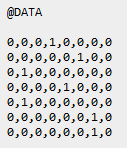
\includegraphics[scale=0.6]{imagenes/data.png}
		\caption{Figura que representa los datos de una apreciación familia.}
	\end{center}
\end{figure}

Estos vectores de entrada representan a cada uno de los ítems, en este caso en particular, a los ítems de la dimensión "Entorno". \\
Cada valor del vector es asociado a los posibles valores en que el profesional puede calificar los ítems. Donde "0" representa que no se marcó ese valor y "1" representa que el profesional a cargo calificó ese ítem según el valor asociado. 

Cada uno de los valores de los vectores de entrada, como aprecia en la Figura \ref{data}, están separados entre ellos por "comas" y al final de cada uno de ellos existirá un salto de espacio para diferenciar que viene otro vector representando el siguiente ítem. \\

\clearpage
\newpage


 \section{Diseño de pruebas}
 En esta sección se proponen las actividades a realizar en las pruebas a la herramienta. Entregando así el diseño de las pruebas unitarias, de integración, de aceptación y finalmente usabilidad.\\ 
\subsection{Método de validación}

 Con el fin de corroborar el cumplimiento de los requerimientos iniciales del Trabajo de Título y corroborar el correcto funcionamiento de la herramienta, se definió un método de validación que pretende establecer para cada etapa de desarrollo del sistema un ítem de pruebas siguiente:\\ 
 \begin{itemize}
 \item Para validar la etapa de implementación o codificación se realizará a Pruebas Unitarias sobre las funcionalidades relevantes de la herramienta por intermedio de pruebas de Caja negra.
 \item Para validar el diseño se efectuarán Pruebas de Sistema e Integración, donde se valida principalmente el desempeño o, respuesta de las funcionalidades criticas del sistema y correcta interacción de las unidades que lo componen.
 \item Para validar la especificación de requerimientos se realizarán Pruebas de Aceptación Usuaria y Usabilidad, donde se determinará la percepción y usabilidad de los usuarios frente al sistema.
\end{itemize}

\clearpage

\subsection{Grupos Muestrales}
Para todas las pruebas descritas en esta sección, se utilizará un conjunto de personas, descritos en la Tabla 4.3. Para las pruebas unitarias y de integración solo se necesitan 2 individuos de prueba, debido a que sólo se evalúa el cumplimiento de los de funciones y sus relaciones. Finalmente para las prueba de aceptación y usabilidad se requiere de un grupo muestral objetivo, que pueda entregar feedback para evaluar la herramienta.\\

\begin{table}[h]
	\begin{tabular}{|l|l|l|}
		\hline
		\textbf{Tipo de Prueba}                & \textbf{Grupo Muestral} & \textbf{Tareas Aplicadas}                  \\ \hline
		Pruebas de Unitarias                   & 2 personas              & Realizar tareas y registrar los resultados \\ \hline
		Pruebas de Integración                 & 2 personas              & Realizar tareas                            \\ \hline
		\multirow{2}{*}{Pruebas de aceptación} & 5 personas              & tareas                                     \\ \cline{2-3} 
		& 10 personas             & realizar tareas                            \\ \hline
		\multirow{2}{*}{Pruebas de Usabilidad} & 5 personas              & tareas                                     \\ \cline{2-3} 
		& 10 personas             & tareas                                     \\ \hline
	\end{tabular}
	\caption{Grupos Muestrales}
\end{table}


\subsection{Pruebas Unitarias}

Las Pruebas Unitarias se utilizará la técnica "Caja Negra". Este técnica implica el ingreso de datos a cada funcionalidad y a la posterior verificación de los datos esperados (Entada y salida). Para llevar a cabo esta técnica se utilizará una plantilla d registro d información obtenida al realizar cada una de las funcionalidades del sistema. La plantilla a utilizar es la siguiente:\\

\begin{table}[htb]
	\begin{tabular}{|l|l|}
		\hline
		\multicolumn{2}{|p{12cm}|}{\textbf{Nombre de la Prueba: Prueba-Nombre Funcionalidad}} \\ \hline
		\textbf{Propósito}                                 &                            \\ \hline
		\textbf{Referecias}                                &                            \\ \hline
		\multicolumn{2}{|c|}{\textbf{Casos de Prueba}}                                  \\ \hline
		\textbf{Entrada Válida}                            &                            \\ \hline
		\textbf{Salida Esperada}                           &                            \\ \hline
		\textbf{Entrada Válida}                            &                            \\ \hline
		\textbf{Salida Esperada}                           &                            \\ \hline
		\textbf{Comentarios}                               &                            \\ \hline
		\textbf{Resultado}                                 &                            \\ \hline
	\end{tabular}
	\caption {Plantilla Caso de Prueba}
\end{table}

\clearpage
\newpage

En la siguiente Tabla se presentan las funcionalidades que serán evaluadas con sus respectivas entradas que debe recibir  y además las salidas esperadas.\\

\begin{table}[h!]
	\begin{tabular}{|p{6cm}|p{6cm}|p{5cm}|}
		\hline
		\multicolumn{3}{|c|}{\textbf{Pruebas Unitarias}}                                                                                                                                                                                                           \\ \hline
		\textbf{Funcionalidad}&\textbf{Entradas} & \textbf{Salidas} \\
		\hline\textbf{CrearUsuario} & \multicolumn{1}{p{6cm}|}{Nombre Usuario, Contraseña, Rut, E-mail, Selección de Tipo de Usuario} & Mensaje con creación de usuario existosa \\ \hline \multicolumn{1}{|p{6cm}|}{\textbf{Modificar Usuario}} & Seleccion del usuario a modificar, Nombre Usuario, Contraseña, E-mail, Selección de Tipo de Usuario & Mensaje de modificación exitosa \\ \hline \textbf{Eliminar Usuario} & Selección del usuario a eliminar y clic en el botón eliminar usuario. & Mensaje de confirmación de la eliminación del usuario\\ \hline	\textbf{Eliminar Usuario Confirmación} & Confirmación de eliminar usuario & Mensaje de eliminación exitosa  \\ \hline \textbf{Ingreso de una apreciación} & Selección de las diferentes dimensiones, asignación de puntajes a los ítems, clic en el botón guardar apreciación & Mensaje de ingreso de apreciación exitosa \\ \hline \textbf{Modificar apreciación} & Selección de la apreciación a modificar, modificar los ítems requeridos, clic en el botón guardar apreciación & Mensaje de modificación de apreciación exitosa \\ \hline
		\textbf{Buscar apreciación} & Ingreso de un nombre de familia a buscar & Lista de las apreciaciones que coinciden con la búsqueda realizada \\ \hline	\textbf{Desplegar información módulo estadística descriptiva} & Selección de la apreciación a desplegar información de estadística descriptiva y clic en el botón generar información & Despliega la información respectiva\\ \hline
		\textbf{Desplegar información módulo minería de datos} & Selección de la apreciación a desplegar información de minería de datos  y clic en el botón generar información & Despliega la información respectiva\\ \hline
		\textbf{Comparar apreciaciones} & Seleccion de las apreciaciones a comparar y clic en el botón generar información & Despliega la información respectiva\\ \hline
	\end{tabular}
	\caption{Funcionalidades, entradas y salidas esperadas.}
\end{table}

 \clearpage
 \newpage

\subsection{Pruebas de integración}

Esta prueba se orienta a verificar que las interfaces entre módulos funcionen correctamente. Para esta prueba se selecciona la estrategia ascendente (Bottom Up), que consiste en realizar un test de las partes individuales con detalle y luego se enlazan para formar componentes más grandes, que a su vez se enlazan hasta que se forma el sistema completo, como se muestra en la Figura.
\subsection{Pruebas de aceptación de usuario}
En esta sección se presentan las pruebas de aceptación de usuario. Con estas pruebas, se busca registrar la experiencia al momento de utilizar las funciones del sistema por parte de nuestros dos usuarios (Administrador y profesional a cargo). Para obtener los registros se utilizarán las plantillas que veremos a continuación, las cuales deben ser completadas con los siguientes parámetros:
\begin{itemize}
	\item Muy difícil de realizar
	\item Difícil de realizar
	\item Opinión neutra
	\item Fácil de realizar
	\item Muy fácil de realizar
\end{itemize}

\begin{table}[h!]
	\centering
	\begin{tabular}{|l|l|}
		\hline
		\multicolumn{2}{|c|}{\textbf{Pruebas de aceptación: Usuario Administrador}}           \\ \hline
		\textbf{Funcionalidad}                                        & \textbf{Apreciación}  \\ \hline
		\textbf{Crear Usuario}                                        & \multicolumn{1}{c|}{} \\ \hline
		\textbf{Modificar Usuario}                                    &                       \\ \hline
		\textbf{Eliminar Usuario}                                     &                       \\ \hline
		\textbf{Eliminar Usuario Confirmación}                        &                       \\ \hline
		\textbf{Ingreso de una apreciación}                           &                       \\ \hline
		\textbf{Modificar apreciación}                                &                       \\ \hline
		\textbf{Buscar apreciación}                                   &                       \\ \hline
		\textbf{Desplegar información módulo estadística descriptiva} &                       \\ \hline
		\textbf{Desplegar información módulo minería de datos}        &                       \\ \hline
		\textbf{Comparar apreciaciones}                               &                       \\ \hline	
	\end{tabular}
	\caption{Plantilla Prueba de aceptación: Usuario Administrador.}
\end{table}
\clearpage
\newpage

\begin{table}[h]
	\centering
	\begin{tabular}{|l|l|}
		\hline
		\multicolumn{2}{|c|}{\textbf{Pruebas de aceptación: Usuario Profesional a Cargo}}    \\ \hline
		\textbf{Funcionalidad}                                        & \textbf{Apreciación} \\ \hline
		\textbf{Ingreso de una apreciación}                           &                      \\ \hline
		\textbf{Modificar apreciación}                                &                      \\ \hline
		\textbf{Buscar apreciación}                                   &                      \\ \hline
		\textbf{Desplegar información módulo estadística descriptiva} &                      \\ \hline
		\textbf{Desplegar información módulo minería de datos}        &                      \\ \hline
		\textbf{Comparar apreciaciones}                               &                      \\ \hline
	\end{tabular}
	\caption Plantilla Prueba aceptación: Usuario Profesional a cargo
\end{table}


\subsection{Pruebas de usabilidad}

Tal como se mencionó en la Sección las pruebas de usabilidad utilizará un conjunto de personas donde cada grupo ejecutará las tareas de las Tablas. Una vez realizadas las tareas los usuarios contestarán el formulario definido en la Tabla 4.12, donde el significado de cada número se encuentra en la Tabla\\




\section{Conclución}  \label{conclusiones}
Incluya análisis crítico sobre  pertinencia del problema, solución propuesta, proyecciones
y estado de avance. Extensión máxima sugerida 2 páginas.\\

\clearpage
\newpage
